\chapter{Detección de marcadores}
\label{deteccionMarcadoresSec}
\section{Introducción}

Como se vio anteriormente, una vez realizada la captura de video del paciente, el primer paso en el procesamiento de las secuencias de video en un sistema de captura de movimiento es reconocer los marcadores en el cuerpo del sujeto, para luego tener la posición de cada uno de ellos en el espacio y a lo largo del tiempo. 

La gran diferencia entre el sistema a implementar y los sistemas modernos es que, por temas de presupuesto, no se utilizarán sensores infrarrojos u otro tipo de tecnología que facilite (o evite) la etapa de segmentación. En lugar de esto se realizará la segmentación por métodos ópticos, es decir, por métodos basados en el estudio de los píxeles de la imagen. 

Debido a las condiciones del laboratorio donde se realizarán las capturas (esto es, marcadores blancos sobre un paciente con ropa oscura, fondo oscuro, e iluminación controlada), el problema de la detección de marcadores puede explicarse en líneas generales, como la detección de círculos blancos de un cierto tamaño sobre fondo oscuro.

\begin{figure}[H]
        \centering
        \subfloat[Captura original]{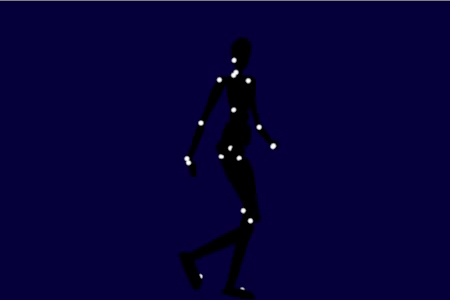
\includegraphics[scale=0.5]{img/peladoFondoAzul.png} %\label{peladoOriginalintro}
        } \hspace{1cm}        
        \subfloat[Segmentación]{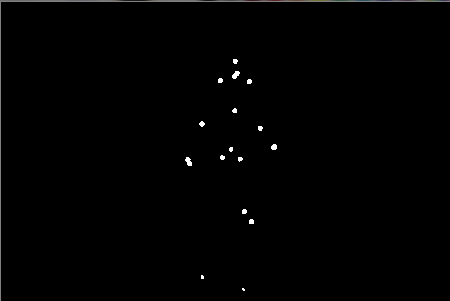
\includegraphics[scale=0.5]{img/peladoFondoAzul_filtro.png}\label{peladoFiltrointro}}

        \subfloat[Detección]{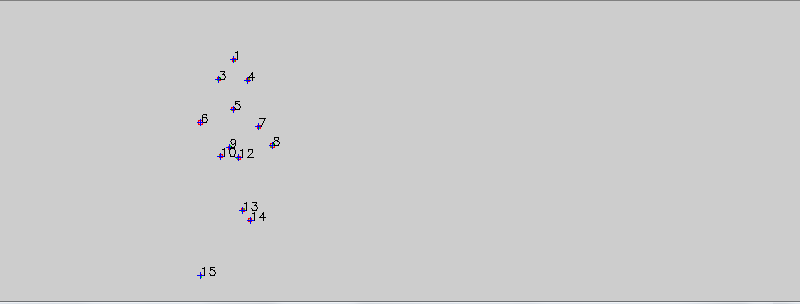
\includegraphics[scale=0.5]{img/peladoFondoAzul_circulos.png} %\label{peladocirculosintro}
        }
  \caption{Ejemplo de funcionamiento del bloque.}
      \label{ejemplotodointro}
\end{figure}

El bloque de detección de marcadores, se puede dividir en dos partes bien definidas: la \textbf{segmentación} y el \textbf{filtrado de objetos hasta obtener los marcadores}. En la Figura \ref{ejemplotodointro} se muestra el resultado del procesamiento de cada parte.

El término segmentar hace referencia, en rasgos generales, a la división de una imagen en múltiples secciones u objetos para su posterior análisis. En otras palabras, la segmentación se encarga de identificar los objetos de importancia dentro de la imagen. 

Algunas de las aplicaciones prácticas de la segmentación son:
\begin{itemize}
\item Pruebas médicas: localización de tumores, medida de volúmenes de tejido, cirugía guiada por computadora, diagnóstico, planificación de tratamiento, estudio de la estructura anatómica
\item Localización de objetos en imágenes satelitales
\item Sensor de  huella dactilar
\item Reconocimiento facial
\item Reconocimiento de iris
\item Sistemas de control de tráfico
\item Visión por computadora
\end{itemize}

El nivel de detalle de este proceso depende del problema a atacar. En este caso la segmentación juega un papel muy importante dentro del sistema ya que, en base a los datos obtenidos en ella se detectarán los marcadores en el cuerpo del paciente, que luego serán utilizados tanto en el tracking como en la reconstrucción 3D. Por otro lado, un error en la detección de la posición de los marcadores será imposible de detectar en etapas posteriores y generará un seguimiento 3D erróneo del mismo. Debido a esto, es recomendable tener la mayor exactitud posible, en especial si se tiene en cuenta que el sistema será utilizado al servicio de la medicina, por lo que deberá tener una precisión mayor que otros sistemas donde el nivel de detalle no juega un papel tan importante (como el Kinect de Microsoft\footnote{http://www.xbox.com/es-ES/Kinect , Noviembre 2014} por ejemplo).

A pesar de lo dicho, no hay que perder el foco que este proyecto busca \textbf{tener una primera versión del sistema de principio a fin con todos los bloques implementados}, aunque esto signifique tener que realizar cada bloque con menor complejidad.

Existen varios métodos a aplicar para realizar la segmentación. Siguiendo lo aclarado en el párrafo anterior se comenzaron probando los más simples y se fue aumentando el nivel de complejidad hasta encontrar un método que se ajuste a los requerimientos. A continuación se describirán dos de los más destacados, entre ellos la generación de umbrales con el método de Otsu \cite{otsu}, que fue el elegido para este sistema. Además se explicará por qué se seleccionó este método en lugar de los otros y cómo funciona el algoritmo implementado. Por último, se mostrarán algunos resultados obtenidos al procesar imágenes sintéticas y reales con este bloque.

\section{Estado del arte}%pag 711, Gonzalez 3º ed
\label{segEstArt}

Dado que la segmentación es la parte más compleja de este bloque, se detallará su estado del arte. Como se mencionó anteriormente, existen varios métodos para realizar la segmentación, en particular los algoritmos para tratar imágenes monocromáticas generalmente se clasifican en dos grupos basados en la intensidad de los píxeles: discontinuidad y similaridad. 

En los algoritmos basados en discontinuidad, se parte de la suposición que los límites de las regiones son suficientemente distintos unos de otros y a su vez del fondo, para permitir detectarlos en base a las discontinuidades de intensidad. Los algoritmos principales en esta categoría son los basados en \textbf{detección de bordes}.

Por otro lado, en los algoritmos basados en similaridad, se busca dividir la imagen en diferentes zonas donde los píxeles de cada una son similares entre sí y comparten ciertas características predefinidas. Los algoritmos más conocidos son los basados en identificación de regiones, como por ejemplo la \textbf{aplicación de umbral}.

A continuación se explican los algoritmos mencionados.

\subsection{Detección de bordes}
\label{detecbordeSec}

Conciste básicamente en la detección de líneas o transiciones en una imagen mediante el procesamiento de los píxeles que la componen. En lo que sigue se explica el detalle de este método, tal como se menciona en el libro \textit{Digital Image Processing de Rafael Gonzalez y Richard Woods} \cite{Gonzalez}.

Así como el difuminado en una imagen (que equivale a hacer un promedio de los píxeles en una zona) puede realizarse mediante la integración, los cambios de intensidad abruptos entre píxeles continuos pueden detectarse utilizando derivadas. Las derivadas de primer y segundo orden son en particular las más indicadas para este propósito.

Las derivadas de una función digital son siempre definidas en términos de diferencia. Hay varias formas de aproximar estas diferencias, pero para lograr detectar bordes de forma correcta es necesario que la aproximación usada para la derivada de primer orden cumpla los siguientes requisitos:

\begin{enumerate}
\item valga cero en áreas de intensidad constante
\item no valga cero al inicio de un escalón o rampa de intensidad
\item no valga cero en los puntos pertenecientes a una rampa de intensidad
\end{enumerate}

De la misma forma, se requiere que la aproximación utilizada para la derivada de segundo orden verifique que:

\begin{enumerate}
\item valga cero en áreas de intensidad constante
\item no valga cero al inicio y al final de un escalón o rampa de intensidad
\item no valga cero en los puntos pertenecientes a una rampa de intensidad
\end{enumerate}

Considerando las propiedades de estas derivadas, se puede concluir que la de primer orden es la más adecuada para detectar bordes más ``gruesos'' y la segunda para detectar los más finos. Así mismo, para detectar puntos aislados la más adecuada es la derivada segunda, lo que no es de sorprender ya que la misma es más sensible que la primera frente a cambios bruscos de intensidad. A raíz de esto, también se concluye que la derivada segunda es la más adecuada para detectar detalles finos (incluido el ruido). También es de destacar que mediante el signo de la la derivada segunda se puede detectar si la transición en un borde (ya sea rampa o escalón) es de luz a oscuridad o viceversa.

Por otro lado, para realizar el procesamiento de las imágenes, se analizan las mismas como matrices numéricas. Una imagen en color, se traduce como tres matrices bidimensionales, una por cada componente cromática (por ejemplo rojo, verde, azul ) siendo las filas y columnas de las matrices, el ancho y largo de la imagen. 
A efectos de simplificar el análisis, se estudian imágenes en escala de grises, lo cual implica trabajar con una sola matriz en vez de tres. En el formato de archivo de imagen TIFF, la escala de grises en 8 bits va de 0 (negro), a 255 (blanco), para cada píxel de la imagen (ver figura \ref{gonz2}).

\begin{figure}[hbt]
\begin{center}
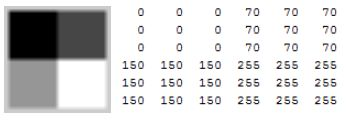
\includegraphics[scale=0.8]{img/02_escala_grises.jpg}
\end{center}
\caption{Imagen en escala de grises y su representación matricial.}
\label{gonz2}
\end{figure}

La herramienta elegida para encontrar tanto la magnitud como la dirección de un borde en la posición $(x,y)$ de la imagen $f$, es el gradiente denotado como ${\nabla}f$ y definido como:

 \begin{equation}
{\nabla}f = grad(f) = \begin{bmatrix}
            {g_x} \\[0.3em]
            {g_y}
            \end{bmatrix} = \begin{bmatrix}
                    {\frac{{\partial}f}{{\partial}x}} \\[0.3em]
                    {\frac{{\partial}f}{{\partial}y}}
                      \end{bmatrix}
 \end{equation}

Para detectar un borde en una imagen resta calcular el gradiente y luego su magnitud para cada píxel Si la superficie es uniforme, esta magnitud será nula (o muy pequeña) y si la superficie varía (por ejemplo, cuando hay un borde de por medio) el valor de la magnitud será alta.

Por otro lado, el gradiente puede ser implementado para todos los valores de $x$ e $y$ pertinentes mediante el filtrado de la imagen $f(x,y)$ con las máscaras de la figura \ref{matrix1d}.

\begin{figure}[H]
\begin{center}
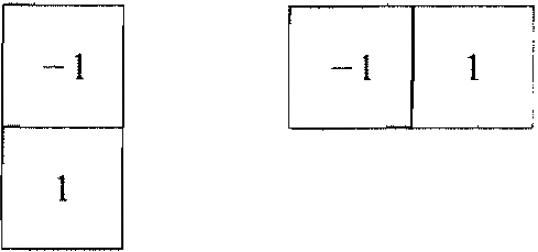
\includegraphics[scale=0.3]{img/matriz1d.png}
\end{center}
\caption{Máscaras de 1 dimensión.}
\label{matrix1d}
\end{figure}

Realizando esto se detectarán los bordes verticales y horizontales de la imagen. Para aumentar el detalle de la detección (por ejemplo para detectar bordes diagonales) es necesario aumentar las dimensiones de las máscaras, por ejemplo, a 2x2 o mejor aún a 3x3.

Existen variedades de máscaras aplicables, entre ellas la de Sobel (ver figura \ref{gonz5}), que presentan beneficios adicionales como la supresión de ruido, manteniendo la característica de detectar los bordes.

\begin{figure}[H]
\begin{center}
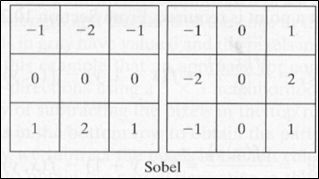
\includegraphics[scale=0.7]{img/08_matriz_sobel.jpg}
\end{center}
\caption{Máscara de Sobel.}
\label{gonz5}
\end{figure}

En la figura \ref{gonz2} se observaba una imagen de 6x6 píxeles y su representación matricial. Al aplicar la máscara de Sobel a la matriz de esta imagen, se detecta la transición entre los 4 niveles de gris mientras que se igualan los niveles constantes. En la figura \ref{gonz6} se pueden observar estos resultados.

\begin{figure}[H]
\begin{center}
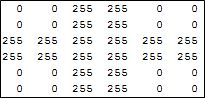
\includegraphics[scale=0.8]{img/09_escala_grises_deteccion_borde.jpg}
\end{center}
\caption{Resultado de aplicar máscaras de Sobel sobre imagen original 6x6.}
\label{gonz6}
\end{figure}

 Este método se puede combinar con otros para mejorar los resultados. Una posibilidad es someter la imagen a un proceso de \textit{smooth} \cite{smooth} -o suavizado- previo a la detección, de esta forma se descartan los bordes pequeños que en general son considerados como ruido. Otra posible combinación para realizar una detección más selectiva es la aplicación de un umbral luego del cálculo del gradiente. Cuando el interés recae tanto en destacar los bordes principales de una imagen como en obtener la mayor conectividad posible, es común que se aplique suavizado y umbral a la vez.

\subsection{Métodos de umbral} %pag 760 del Gonzalez
\label{umbralSec}

Los métodos del valor umbral son un grupo de algoritmos cuya finalidad es segmentar los objetos de una imagen en función de un rango de valores. La pertenencia de un píxel a cierto segmento se decide mediante la comparación de alguna propiedad unidimensional del mismo (por ejemplo su nivel de gris o nivel de luminosidad) con cierto valor umbral. Dado que esta comparación de valores se realiza individualmente para cada píxel, al método del valor umbral se le considera un método de segmentación orientado a píxeles.

Por lo tanto, mientras en los métodos de detección de bordes las regiones eran identificadas encontrando primero segmentos de borde y luego tratando de unir los mismos para formar bandas, en los métodos de umbral se trata de separar la imagen directamente en regiones basándose en la intensidad de estos píxeles y/o en otras propiedades, reduciendo el problema a encontrar el umbral correcto.

En la figura \ref{gonz3} se observa el resultado de aplicar el método de umbral a la figura \ref{gonz2} con un umbral de 200.

\begin{figure}[H]
\begin{center}
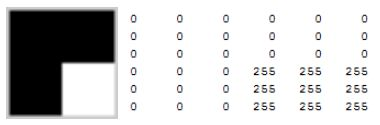
\includegraphics[scale=0.8]{img/03_escala_grises_umbral.jpg}
\end{center}
\caption{Resultado de aplicar un umbral de valor 200.}
\label{gonz3}
\end{figure}


%%%%%%%%%%%%%%%Segmentación de 3 clases%%%%%%%%%%%%%
En este ejemplo se aplica el proceso más simple de generación de umbrales, sin embargo, en la mayoría de los casos ajustar el histograma de una imagen a esta forma no da tan buenos resultados. Para estas situaciones se recurre a la \textit{umbralización múltiple}, donde un punto $(x,y)$ se puede clasificar en varias clases dependiendo de la complejidad de la imagen.

Cuando la distribución de las intensidades entre objeto y fondo se encuentran lo suficientemente distinguidas, es posible utilizar un solo umbral global aplicable en toda la imagen. Por otro lado, para aplicaciones donde el valor del umbral debe ir cambiando para una secuencia de imágenes, es recomendable utilizar algún método para calcular el valor del mismo automáticamente. En base a los factores que afectan la imagen y a las restantes características de la misma, se han implementado distintas formas de obtener el valor de umbral. El siguiente algoritmo iterativo muestra un ejemplo sencillo de como calcular el umbral:

\begin{enumerate}
\item Seleccionar un umbral inicial $T$ estimado.
\item Segmentar la imagen utilizando $T$. Esto producirá dos conjuntos de píxeles, los que estén por encima del umbral ($C_1$), y los que estén por debajo ($C_2$).
\item Calcular el promedio de las intensidades ($m_1$ y $m_2$) de los píxeles en $C_1$ y $C_2$ respectivamente.
\item Calcular un nuevo umbral $T = \frac{1}{2}(m_1 + m_2)$.
\item Repetir los pasos 2 a 4 hasta que la diferencia entre los umbrales $T$ de sucesivas iteraciones sea menor a un ${\Delta}T$ definido anteriormente.
\end{enumerate}

Los principales métodos existentes para obtener el valor del umbral están listados en el survey de Mehmet Sezgin \cite{surveyThreshold}, en el cual se clasifica estos métodos en las siguientes categorías:
\begin{itemize}
\item Basados en la forma del histograma.
\item Basados en agrupamiento.
\item Basados en la entropía de las regiones.
\item Basados en los atributos de los objetos.
\item Espaciales.
\item Locales.
\end{itemize}

Entre los cuarenta métodos exhibidos en este paper, se encuentra el método de Otsu\cite{otsu}. El mismo se encuentra dentro de los métodos basados en agrupamiento y es uno de los más utilizados en segmentación por umbral debido a su eficacia y simplicidad. Utiliza técnicas estadísticas para resolver el problema. En particular se utiliza la varianza que, como es sabido, es una medida de la dispersión de valores (en este caso se trata de la dispersión de los niveles de gris).

%\textbf{Uso del difuminado (Smooth) para mejorar la umbralización}

%Como se comentó en la sección \ref{detecbordeSec}, es común utilizar métodos de smoothing y umbral en simultáneo para mejorar el proceso de segmentación ya que el smoothing es una buena técnica para eliminar el ruido previo a aplicar el umbral. De hecho, cuanto más alto sea el nivel de \textit{smoothing} en una imagen, más errores en los bordes se anticiparán al segmentar.


\section{Justificación del algoritmo elegido}

En un principio, se manejó la idea de tomar como base una implementación existente y adaptarla para el propósito de este proyecto. Sin embargo, en la etapa de investigación se encontró que no hay muchos sistemas de código abierto disponibles, y los que se encontraron necesitan muchos ajustes para llegar a cubrir las necesidades de este trabajo. En particular, para la segmentación se encontraron varias implementaciones de algoritmos, pero ninguna se ajusta a los requerimientos del proyecto. Por esta razón se decidió implementar un algoritmo conocido, que aplique la teoría de la sección \ref{segEstArt}.

De los métodos nombrados en la sección anterior, si se piensa en los requerimentos del sistema, la detección de bordes presenta alguna desventajas frente a la detección por umbral. En primer lugar, si bien en los objetos a detectar hay bordes, los mismos no son tan nítidos debido al difuminanado natural que impone la forma esférica de los marcadores. Este aspecto puede afectar negativamente la detección de bordes ya que el contraste entre un pixel y su vecino no es tán pronunciado, sin embargo en la segmentación por umbral, esta característica simplemente afectaría el tamaño de la esfera segmentada en función del valor del umbral impuesto. Además la detección de bordes presenta otros problemas que la umbralización no, y que a efectos de este proyecto es mejor evitar, por ejemplo, los bordes detectados usualmente quedan desconectados al aplicar detección de bordes e integrarlos es bastante costoso. Por esto, y debido a sus propiedades intuitivas, simplicidad en la implementación y a su rapidez computacional, se eligió utilizar un método de umbral para implementar el bloque de \emph{Segmentación}. En particular se eligió el método de Otsu \cite{otsu} de tres clases ya que ofrece un buen compromiso entre simplicidad y eficacia como se verá más adelante. 

Para la elección del número de clases se tuvo en cuenta las características de la captura de video a procesar. Usar el número de clases incorrecto afecta en gran medida la segmentacióm. En un principio se podría suponer que cuánto mayor es el número de clases más precisa será la segmentación, sin embargo esto no es correcto. Un error típico al usar un número mayor al adecuado de clases es tener un único objeto segmentado en varios más pequeños. Por otro lado, utilizar un número menor de clases también es causa de errores. Por ejemplo, al utilizar 2 clases, se está asumiendo que el fondo es uniforme lo que, como se verá más adelante, no sucede en las capturas de video de este sistema.

Para realizar esta elección se tuvo en cuenta que las capturas a procesar serán realizadas en un ambiente controlado y, siguiendo con la filosofía de priorizar la completitud del sistema frente a la eficacia del mismo, no se tuvo como prioridad para esta primera etapa implementar un método de mayor complejidad que sea más robusto frente a ciertos tipos de ruidos o características que se pueden dar en otro tipo de capturas (iluminación, fondo, ropa del paciente, etc.). 

Con el método de Otsu \cite{otsu} se pretende, a partir del histograma de la imagen, separar los píxeles de la misma en 3 niveles encontrando dos umbrales que los separen. Trabajar con tres clases permite ser un poco más flexible con los contrastes entre los marcadores y el resto de la imagen por lo que no sería estrictamente necesario, por ejemplo, que el traje del paciente y el fondo sean del mismo color.

El bloque de segmentación de este sistema fue implementado en el lenguaje C++, debido a que es uno de los lenguajes de programación que cuenta con mayor cantidad de recursos para procesamiento de imágenes. En particular, se utilizaron las librerías OpenCV \cite{opencv} y CVBlob \cite{cvblob} ya que funcionan para las plataformas principales de PC y dispositivos móviles, y están diseñadas para tener una gran eficiencia computacional en las implementaciones. Además, estas librerías son de las más populares dentro de las de código abierto con estas características, lo que implica tener una comunidad activa de usuarios muy grande.

Por otro lado, C++ es un lenguaje relativamente antiguo por lo que implementar el algoritmo con el mismo implicó más esfuerzo (por ejemplo, en el manejo de la memoria) que de haber utilizado un lenguaje más nuevo. Esto contribuyó a impedir la implementación de un algoritmo más complejo.

Finalmente, la justificación de la realización del algoritmo para el bloque de segmentación puede entenderse desde dos puntos de vista: 
\begin{itemize}
 \item Por un lado, se elaboró un algoritmo de una complejidad relativamente baja como se estableció en los requerimientos, pero que cubre todas las características necesarias para esta clase de sistema. En la sección \ref{resultadosyanalisissegmentacion} se verá que los resultados obtenidos son buenos y el error cometido está dentro de los márgenes que aseguran el buen funcionamiento del sistema.
 \item Por otro lado, a pesar de que el estado del arte de segmentación presenta una gran cantidad de algoritmos, el estado del arte ``industrial'' está bastante más atrasado del estado del arte referente a investigaciones debido al tiempo que implica realizar una nueva implementación o la dificultad para conseguir una. Por esto, implementar una primera versión del sistema con el algoritmo de segmentación elegido no está muy alejado de los que se usan actualmente. Nuevamente, es importante aclarar que este bloque (como el resto de los bloques) está implementado de forma tal que en un futuro se pueda optimizar tanto como se quiera, sin afectar el resto de los bloques del sistema. Esto da la posibilidad de poder modificar el sistema no solo para mejorar la segmentación sino también para robustecerla permitiendo, entre otras cosas, realizar capturas fuera de las condiciones del laboratorio como puede ser en la práctica de algún deporte.
\end{itemize}


\section{Algoritmo}

\subsection{Fundamento teórico }
\label{fundamentoteoseg}

A continuación, se presentan algunos conceptos básicos necesarios para entender la implementación de un algoritmo con segmentación por umbral:

\begin{figure}[hbt]
\begin{center}
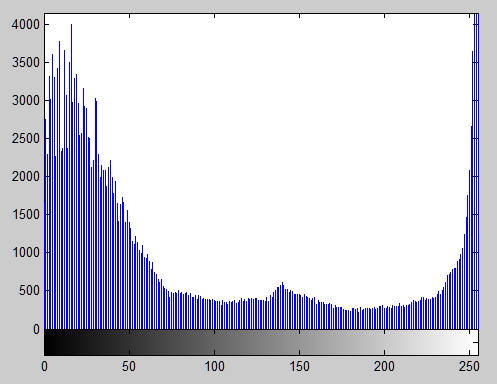
\includegraphics[scale=0.7]{img/otsu2.png}
\end{center}
\vspace{-0.5cm}
\caption{Histograma de intensidad de una imagen.} 
\label{otsuFruta}
\end{figure}



Considerando la figura \ref{otsuFruta} \footnote{\textcolor{blue}{\underline{\url{ http://deploy.virtual-labs.ac.in/labs/cse19/theory.php?exp=segment}}}}  como el histograma de intensidad de una imagen, $f(x,y)$, se puede apreciar que la misma está compuesta por un objeto u objetos iluminados de aproximadamente la misma intensidad y un fondo oscuro. De esta manera, se definen en este histograma dos campanas bien determinadas. La manera más obvia de extraer los objetos del fondo es seleccionando un umbral $T$ que separe estas dos campanas y por lo tanto cualquier punto $(x,y)$ de la imagen que cumpla $f(x,y) > T$ será un punto perteneciente al objeto mientras que el resto son puntos pertenecientes al fondo. De acuerdo a lo anterior, la imagen segmentada puede definirse de la siguiente manera.

\begin{equation}
g(x,y) = \left\{
\begin{array}{l}
\displaystyle 1{\qquad}si{\quad}f(x,y) > T\\
\displaystyle 0{\qquad}si{\quad}f(x,y)\;{\leq}\;T
\end{array} 
\right.
\label{eq:xdef}
\end{equation}

Si $T$ toma un valor constante en toda la imagen, al proceso se le llama \textit{umbralización global}. Por otro lado, si $T$ cambia en una imagen el proceso es llamado \textit{umbralización variable}. A veces se utiliza el término \textit{umbralización local o regional} en la umbralización variable cuando el valor de $T$ en un punto $(x,y)$ depende de las propiedades de los puntos al rededor de $(x,y)$.

\begin{figure}[hbt]
\begin{center}
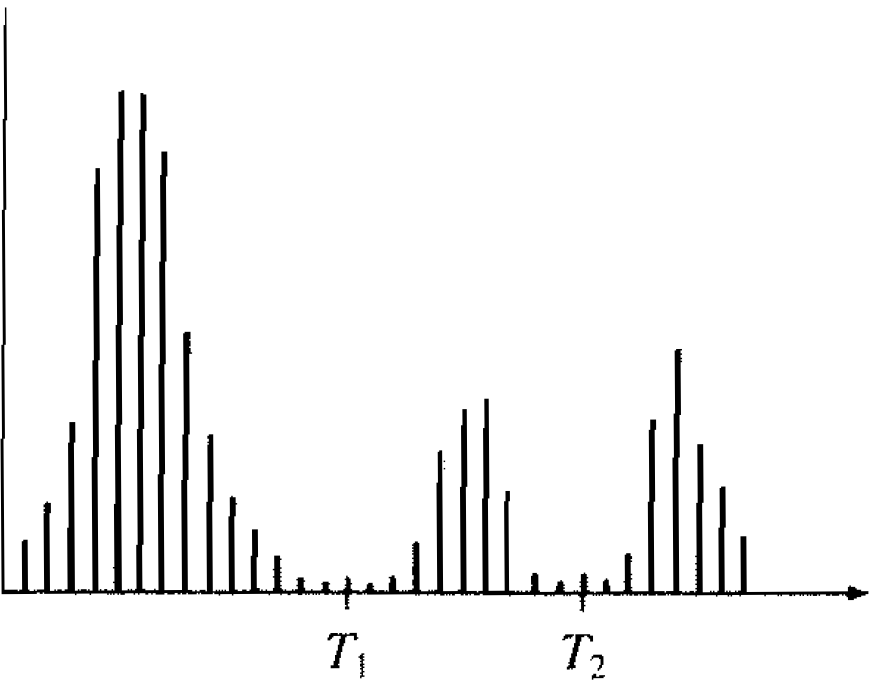
\includegraphics[scale=0.35]{img/hist3clases.png}
\end{center}
\vspace{-0.5cm}
\caption{Histograma de intensidad de tres clases \cite{segment}.}
\label{hist3class}
\end{figure}

En la figura \ref{hist3class} se puede ver el histograma de una imagen con 3 clases dominantes correspondientes, por ejemplo, a un objeto brillante, otro un poco menos brillante y un fondo oscuro. En este caso la umbralización de 3 clases clasificará el punto $(x,y)$ como perteneciente al fondo si $f(x,y){\leq}T_1$, perteneciente a un objeto si $T_1 < f(x,y){\leq}T_2$ y perteneciente al objeto más brillante si $f(x,y)>T_2$. Por lo tanto, la imagen segmentada será de la forma:

\begin{equation}
g(x,y) = \left\{
\begin{array}{l}
\displaystyle a{\qquad}si{\quad}f(x,y) > {T_2}\\
\displaystyle b{\qquad}si{\quad}{T_1} < f(x,y)\;{\leq}\;{T_2}\\
\displaystyle c{\qquad}si{\quad}f(x,y)\;{\leq}\;{T_1}
\end{array} 
\right.
\label{eq:xdef3}
\end{equation}

donde $a,b$ y $c $ son tres valores distintos de intensidad.

Observando los histogramas anteriores, puede verse que la efectividad de la umbralización está directamente relacionada con el ancho y la profundidad de los valles que separan las distintas clases. Siguiendo esto, los factores claves que afectan directamente al tamaño de estos valles son:
\begin{itemize}
\item Separación entre picos: cuanto más separados, mejor posibilidad de segmentar correctamente.
\item Ruido de la imagen.
\item La relación entre los tamaños de los objetos y el fondo.
\item La uniformidad de la iluminación.
\item La uniformidad de las propiedades de reflexión de la imagen.
\end{itemize}

Es de destacar que, si bien no resulta tan evidente como pasa con el ruido de la imagen, la iluminación y las propiedades de reflexión juegan un papel clave para obtener una segmentación efectiva y por lo tanto controlar estos parámetros debe ser prioridad si se quiere obtener una buena segmentación. Cuando no es posible controlarlos, existen tres aproximaciones básicas que se pueden realizar para mejorar los resultados: corregir el patrón de sombras directamente, corregirlo mediante algún proceso ya establecido (por ejemplo utilizando la transformada top-hat \cite{tophat}) o aplicar un umbral variable tal como fue mencionado anteriormente.

%%%%%%%%%%%%%%%%%%%%%%%%%%%%%%%%%%%%%%%%%%%%%%%%%%%%%
%\vspace{10 mm}
\subsubsection{Umbral de Otsu}

El método de Otsu \cite{otsu} calcula el valor umbral de forma tal que la dispersión dentro de cada segmento sea lo más pequeña posible, pero al mismo tiempo sea lo más alta posible entre segmentos diferentes. Para ello se calcula el cociente entre ambas varianzas (para el caso de dos clases) y se busca un valor umbral para que este cociente sea máximo.

Dicho de otra modo, se puede ver al proceso de umbralización como un problema estadístico cuyo objetivo es minimizar el error promedio que se produce al asignar los píxeles de la imagen a dos o más clases. La solución a este problema es conocida como \textit{regla de decisión de Bayes \cite{bayes}}. Sin embargo aplicar esta regla no es tan sencillo, ya que estimar la densidad de probabilidad de cada clase no es simple. El método de Otsu es considerado una de las mejores aproximaciones a esta solución, ya que maximiza la ``varianza intermedia entre clases'' (\textit{between class variance}\footnote{diferencia entre la varianza total y la suma de las varianzas de cada clase\cite{betweenvarianze}}) que es una medida muy utilizada en problemas de discriminación estática, lo que permite obtener un umbral óptimo. A esto se le suma la ventaja de que todos los cálculos realizados en el método se realizan sobre el histograma de intensidades que es muy fácil de obtener.


La ``varianza intermedia entre clases'' puede escribirse como

\begin{equation}
{\sigma}_B^2 = P_1(m_1-m_G)^2 + P_2(m_2-m_G)^2 = P_1P_2(m_1-m_2)^2 = \frac{(m_GP_1 - m)^2}{P_1(1-P_1)}
\label{betvarec}
\end{equation}

donde $P_1$ y $P_2$ son las probabilidades de que un píxel sea asignado a la clase $1$ y $2$ respectivamente, $m_1$ y $m_2$ son las medias de las intensidades de cada una de estas clases. Además, $m(k)$ es la media (intensidad promedio) acumulada  hasta el nivel $k$ y $m_G$ es la intensidad media (intensidad global promedio) de la imagen en su totalidad:
\begin{equation}
m(k) = \sum_{i=0}^{k}ip_i
\label{mediacumulativa}
\end{equation}

\begin{equation}
m_G(k) = \sum_{i=0}^{L-1}ip_i
\label{mediaglobal}
\end{equation}

y considerando que k es el umbral que separa la clase $1$ de la clase $2$, $P_1$ puede escribirse como

\begin{equation}
 P_1(k) = \sum_{i=0}^kp_i 
 \label{peuno}
\end{equation}

donde $p_i$ es la cantidad normalizada de píxeles de la imagen que tienen intensidad $i$.

Por lo que la ecuación \ref{betvarec} también queda dependiendo del umbral $k$:

\begin{equation}
{\sigma}_B^2(k) = \frac{(m_GP_1(k) - m(k))^2}{P_1(k)(1-P_1(k))}
\label{betvarec2}
\end{equation}

Para el caso de umbralización con múltiples clases ($K$ clases), la varianza intermedia vale:

\begin{equation}
  {\sigma}_B^2(k) = \sum_{k=1}^{K}P_k(m_k-m_G)^2
  \label{betvarec3}
\end{equation}

donde $$P_k=\sum_{i{\epsilon}C_k}P_i$$ $$m_k = \frac{1}{P_k}\sum_{i{\epsilon}C_k}ip_i$$ y $m_G$ es la ganancia global como se definió anteriormente. Esta umbralización implica tener $K-1$ umbrales.

A modo de ejemplo, para 3 clases (3 niveles de intensidades separadas por 2 umbrales) la ``varianza intermedia entre clases'' queda:
\begin{equation}
  {\sigma}_B^2(k) = P_1(m_1 - m_G)^2 + P_2(m_2 - m_G)^2 + P_3(m_3 - m_G)^2
\end{equation}

donde $$P_1=\sum_{i=0}^{k_1}p_i$$ $$P_2=\sum_{i=k_1+1}^{k_2}p_i$$  $$P_3=\sum_{i=k_2+1}^{L-1}p_i$$ y $$m_1 = \frac{1}{P_1}\sum_{i=0}^{k_1}ip_i$$  $$m_2 = \frac{1}{P_2}\sum_{i=k_1+1}^{k_2}ip_i$$  $$m_3 = \frac{1}{P_3}\sum_{i=k_2+1}^{L-1}ip_i$$

Además, como en el caso de 2 clases, se dan la siguientes relaciones:
\begin{equation}
  P_1m_1 + P_2m_2 + P_3m_3 = m_G
\end{equation}
y
\begin{equation}
  P_1+P_2+P_3 = 1
\end{equation}

Luego, aplicando lo visto acerca del umbral de Otsu, se tiene que el umbral óptimo $k^*$ es el valor de $k$ que maximiza \ref{betvarec2} (para el caso de múltiples clases, serían los valores de $k_k^*$ que maximizan \ref{betvarec3}). Para encontrar $k^*$ basta con evaluar la ecuación \ref{betvarec2} para todos los valores de $k$ válidos\footnote{ todos los $k$ enteros tal que $0{\leq}k{\leq}L-1$ (con $L-1$ nivel de intensidad máximo de la imagen) que verifiquen $0<P_1(k)<1$ } y seleccionar el valor de $k$ que maximiza dicha ecuación. Si el máximo ${\sigma}_B^2(k)$ se da para varios $k$, $k^*$ se calcula como el promedio de los $k$ que dan dicho valor.

Para el ejemplo del algoritmo de 3 clases, se deberían encontrar los valores de $k_1$ y $k_2$ que maximicen la varianza entre clases. Para ello, se evalúa la ecuación \ref{betvarec3} para todos los pares $(k_1,k_2)$ posibles, es decir: $(k_1,k_2) tq 0<k_1<k_2<L-1$.

Algo importante a destacar es que este método es poco costoso en términos computacionales ya que el máximo numero de $k's$ para los que hay que evaluar la ecuación \ref{betvarec2} es $L$, que corresponde a la cantidad de niveles de intensidad de la imagen.

En resumen, el \textit{algoritmo de Otsu} se puede implementar de la siguiente manera:
\begin{enumerate}
 \item Realizar el histograma de la imagen, donde cada componente corresponde a un nivel de intensidad (con un total de $L$ niveles)
 \item Calcular la probabilidad $P_1(k)$ con la ecuación \ref{peuno} para $k=0,1,2,...,L-1$.
 \item Calcular la media $m(k)$ con la ecuación \ref{mediacumulativa} para $k=0,1,2,...,L-1$.
 \item Calcular la media global $m_G$ con la Ecuación \ref{mediaglobal}.
 \item Calcular la ``varianza intermedia entre clases'' (\textit{between-class variance}), ${\sigma}_B^2(k)$, como se muestra en la ecuación \ref{betvarec2} (o \ref{betvarec3})  para $k=0,1,2,...,L-1$.
 \item A partir del punto anterior, obtener el umbral de Otsu $k^*$ como el valor de $k$ (o los valores de $k_k$ para el caso de múltiples clases) que maximiza ${\sigma}_B^2(k)$.
\end{enumerate}

%\vspace{8 mm}
\subsubsection{Momentos y excentricidad \cite{imageMoments}} 

Los momentos geométricos son propiedades numéricas que se pueden obtener de una determinada imagen, los cuales proporcionan una alternativa interesante para la representación de la forma de un objeto. Tienen en cuenta todos los píxeles de la imagen, no sólo los bordes y se pueden clasificar en:

\begin{itemize}
\item Momentos simples
\item Momentos centrales
\item Momentos centrales normalizados
\end{itemize}

Los \textit{momentos simples} se emplean para obtener otros momentos, pero también dan información por sí mismos. El momento de orden $(p+q)$ se calcula como $$m_{pq}={\int}{\int}x^py^qf(x,y)dxdy$$ donde $f(x,y)$ es una función continua En el espacio discreto se calculan: $$M(p,q))={\sum}_x{\sum}_yx^py^qf(x,y)$$

A partir de esta definición se puede ver, por ejemplo, que el momento simple de orden 0 representa el área de la figura en imágenes binarias, ya que es la suma de los valores de todos los píxeles: $$M(0,0) = {\sum}_x{\sum}_yf(x,y)$$

Por otro lado, los \textit{momentos centrales} son utilizados para reconocer figuras dentro de una imagen, independientemente de su posición. Se calculan como $${\mu}_{pq}={\int}{\int}(x-X)^p(y-Y)^qf(x,y)$$ o para el espacio discreto como $${MC}_{pq}={\sum}{\sum}(x-X)^p(y-Y)^qf(x,y)$$ donde $(X,Y)$ corresponden al centro de masa de la figura (centroide) y se calcula con los momentos simples de orden $0$ y $1$: $$X=\frac{M(1,0)}{M(0,0)} \hspace{5 mm} Y=\frac{M(0,1)}{M(0,0)}$$

Finalmente, los \textit{momentos centrales normalizados}, permiten reconocer figuras dentro de una imagen, independientemente de su posición y de su tamaño. Para ello, se normalizan los momentos centrales con el momento de orden $0$, obteniendo así figuras independientes de la escala: $$MCN(p,q) = \frac{MC(p,q)}{MC^{\beta}(0,0)}$$ donde ${\beta}=\frac{p++q}{2}+1$.

El reconocimiento de la forma de un objeto, se analiza a partir de los momentos de orden 2 (es decir, $p+q=2$). En ellos, la densidad de la figura se multiplica por distancias al cuadrado desde el centro de masas o centroide. Así por ejemplo, con los 3 momentos centrales de segundo orden ($MC(0,2)$, $MC(2,0)$, $MC(1,1)$) se forman las componentes del tensor de inercia o matriz de rotación. A partir de estas componentes, también se puede calcular el ángulo de rotación de la figura alrededor de su centro de masas y la excentricidad. Esta última, se calcula a partir de la ecuación \ref{excentec}, donde $n_{20}$, $n_{02}$ y $n_{11}$ son los momentos centrales normalizados de orden 2.

\begin{equation}
e = \sqrt{1-\frac{\frac{n_{20}+n_{02}}{2}-\sqrt{4n_{11}^2+\frac{(n_{20}-n_{02})^2}{2}}}{\frac{n_{20}+n_{02}}{2}+\sqrt{4n_{11}^2+\frac{(n_{20}-n_{02})^2}{2}}}}
\label{excentec}
\end{equation}

\subsection{Implementación}
\label{implementSegment}

\begin{figure}[H]
\hspace{-1.5cm}
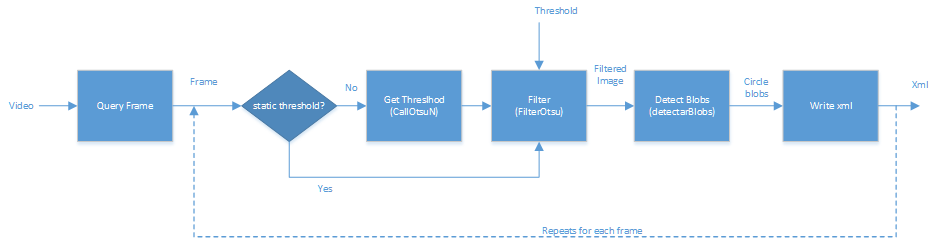
\includegraphics[scale=0.7]{img/diagrama_segmentacion.png}

\caption{Diagrama de flujo del algoritmo de segmentación.}
\label{diagramaSegmentacion}
\end{figure}

En la figura \ref{diagramaSegmentacion} se presenta un diagrama dónde se observa el flujo del algoritmo de segmentación realizado. Los nombres que aparecen entre paréntesis dentro de algunos bloques son los nombres de las funciones dentro del código que implementan cada bloque. 

El algoritmo realiza la segmentación siguiendo el siguiente proceso:

\begin{enumerate}
  \item Se recibe como entrada un video y este es separado en cada uno de sus cuadros a través del bloque \emph{Query Frame}.
  \item Se toma un cuadro, y se calcula el umbral de Otsu con el bloque \emph{Get Threshold}. Si al comenzar la segmentación es ingresado un umbral fijo, este paso se saltea.
  \item Con el umbral calculado (o ingresado), se filtra el cuadro en el bloque \emph{Filter}.
  \item A partir de la imagen filtrada, se identifican los marcadores con el bloque \emph{Detect blobs}.
  \item Se escribe la posición de los marcadores detectados para este cuadro en un archivo con formato xml.
  \item Se toma el siguiente cuadro y se repite el proceso a partir del paso 2.
\end{enumerate}


El bloque \emph{Query Frame} es implementado mediante las funciones \emph{cvCaptureFromAVI} y \emph{cvQueryFrame}, las cuales pertenecen a la librería \emph{OpenCV} \cite{opencv}.


Por otro lado, el bloque \emph{Get Threshold} contiene una implementación del algoritmo de Otsu de $N$ clases \cite{implementacionOtsu}, cedida por Matías Tailanian y Juan Cardelino, que es utilizada con $N=3$. Se utilizó esta implementación ya que la implementación que hay en la librería OpenCV es de dos clases y tampoco se encontraron otras implementaciones del algoritmo para 3 clases en internet.

 Como se vio en la sección \ref{umbralSec}, este método devuelve 2 umbrales de los cuales se tomará el mayor de ellos, dado que las hipótesis del problema establecen que la adquisición de video debe realizarse sobre fondo oscuro y con el paciente utilizando ropa oscura, de forma tal que los marcadores (que son de color blanco) sean los elementos más claros en la imagen.

En la figura \ref{diagramaumbralizacion}, se observa un diagrama que describe el funcionamiento del bloque \emph{Filter}. Este bloque es el encargado de filtrar la imagen según la intensidad de los píxeles y está implementado por la función \emph{FilterOtsu}, que recibe como parámetros de entrada una imagen (uno de los cuadros de la secuencia) y el umbral a utilizar para el filtrado. Primero se le aplica a la imagen un difuminado (\textit{smoothing}) con un filtro de mediana, con el objetivo de reducir el ruido. Luego se cambia el el espacio de colores de la imagen de RGB a HSV ya que este último es más adecuado para realizar segmentación basada en la intensidad de los píxeles \cite{HSV}. Por último, se filtra la imagen con el umbral ingresado, utilizando la función \emph{cvThreshold} de la librería OpenCV. Esta función compara la intensidad de cada píxel de la imagen con el valor del umbral estableciendo un nuevo valor de intensidad: $0$\footnote{negro en el espacio HSV.} para los píxeles que originalmente tenían intensidad menor al umbral y $255$\footnote{blanco en el espacio HSV.} para los que originalmente presentaban intensidad mayor.

\begin{figure}[ht!]
\begin{center}
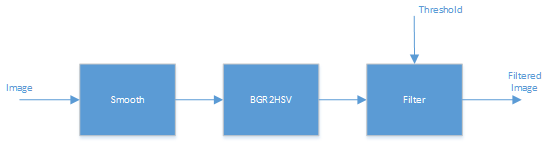
\includegraphics[scale=0.7]{img/diagrama_umbralizacion.png}
\end{center}
\caption{Diagrama de flujo del bloque de umbralización.}
\label{diagramaumbralizacion}
\end{figure}

En la figura \ref{ejemploUmbralizacion}, se puede ver un ejemplo de los resultados de procesar una imagen sintética de la base de datos, con el bloque \emph{Filter}. Se puede ver que la intensidad de los píxeles azules y negros queda por debajo del umbral, mientras que los píxeles blancos quedan por encima. %SE PODRÍA PONER EL HISTOGRAMA

\begin{figure}[ht!]
        \hspace{-1cm}
        \subfloat[Captura original de una secuencia sintética.]{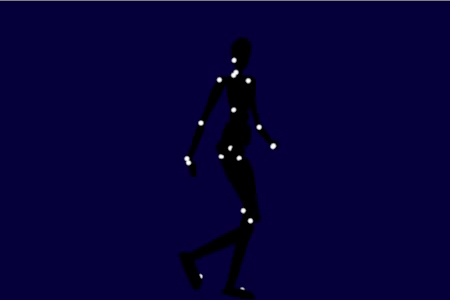
\includegraphics[scale=0.65]{img/peladoFondoAzul.png} %\label{peladoOriginal}
        } \hspace{0.1cm}        
        \subfloat[Imagen filtrada con el umbral de Otsu.]{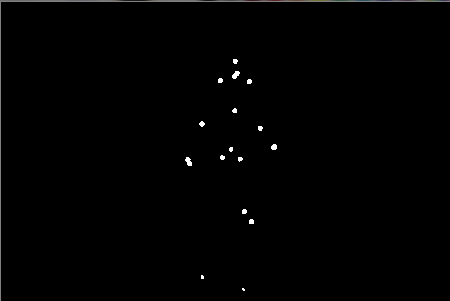
\includegraphics[scale=0.65]{img/peladoFondoAzul_filtro.png}\label{peladoFiltro}}
  \caption{Entrada y salida del bloque de umbralización.}
      \label{ejemploUmbralizacion}
\end{figure}

Como se ve en la figura \ref{peladoFiltro}, para el caso ideal todos los píxeles resultantes del filtrado corresponden a los marcadores en el paciente. En la práctica, no siempre sucede esto, por lo que luego de obtenidos los mismos debe hacerse una diferenciación entre los marcadores y el resto de los píxeles detectados.

El funcionamiento del bloque \emph{Detect blobs} es descrito por el diagrama de la figura \ref{diagramadetectblobs}. Este bloque recibe como entrada la imagen previamente filtrada por el bloque \emph{Filter} y da como salida una imagen con los marcadores detectados e identificados. En primer lugar, se identifican todos los blobs\footnote{Binary Large Objects \cite{defBlob}} de la imagen filtrada con el bloque \emph{Find blobs}, que es implementado por la función \emph{cvLabel} de la librería CVBlob \cite{cvblob}. Cuando se hace referencia a ``identificar todos los blobs'', se refiere a identificar cada grupo de píxeles blancos continuos de la imagen filtrada como un objeto (un blob) único. En la figura \ref{peladoBlobs}, se ve el resultado de procesar la imagen \ref{peladoFiltro} con el bloque \emph{Detect blobs}. 

Luego, si se ingresó la opción para filtrar por área, los blobs \cite{defBlob} detectados se filtran por área máxima y/o mínima mediante la función \emph{cvFilterByArea} perteneciente a la librería CVBlobs \cite{cvblob}. 

\begin{figure}[H]
\hspace{-1.5cm}
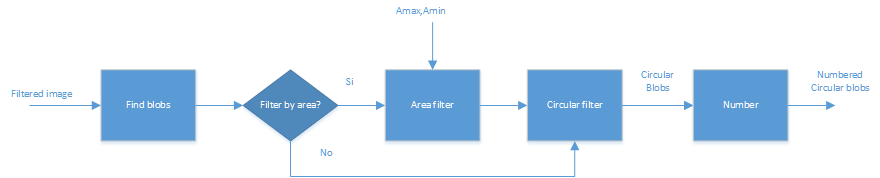
\includegraphics[scale=0.7]{img/detectBlobs_diagrama.png}
\caption{Diagrama de flujo del bloque de detección de blobs.}
\label{diagramadetectblobs}
\end{figure}

Siguiendo el flujo, la imagen con blobs ingresa al bloque \emph{Circular filter}, se haya filtrado por área o no, donde se descartan los blobs que no tienen forma circular. Para ello, se realiza un cálculo basado en la excentricidad\footnote{Parámetro asociado con cada sección cónica. Es una buena medida de cuánto se diferencia dicha sección de ser circular. Así, un círculo tendrá excentricidad 0, una elipse entre 0 y 1, para una parábola valdrá 1 y para una hipérbola será mayor a 1 \cite{excentricidad}. } de los objetos y en los momentos de la imagen. Estas propiedades se explicaron en la sección \ref{fundamentoteoseg}.

De los blobs detectados en un cuadro, los que tendrán forma aproximadamente circular serán los que tengan el valor de la excentricidad más cercana a $0$. Observando la ecuación \ref{excentec}, se puede ver que $e{\rightarrow}0$ si $$\sqrt{4n_{11}^2+\frac{(n_{20}-n_{02})^2}{2}}\ {\rightarrow}\ 0$$ por lo que una buena medida de qué tan circular es un blob puede ser evaluar $n_{11}$ y $n_{20}-n_{02}$ y ver qué tan chico son sus valores en comparación con $n_{20}+n_{02}$.

Precisamente, para la implementación del bloque \emph{Circular Filter}, se evalúa para cada blob $$\frac{n_{11}}{n_{20}+n_{02}}< A$$ y $$\frac{n_{20}-n_{02}}{n_{20}+n_{02}}< B$$ donde $A$ y $B$ son constantes, que cuanto más cercanas a $0$ sean más preciso harán el filtro. En la figura \ref{ejemplofiltrocirc} se observa un ejemplo para las constantes $A = 0.1$ y $B = 0.3$.

\begin{figure}[H]
        \centering
        \subfloat[Entrada - Filtro circular.]{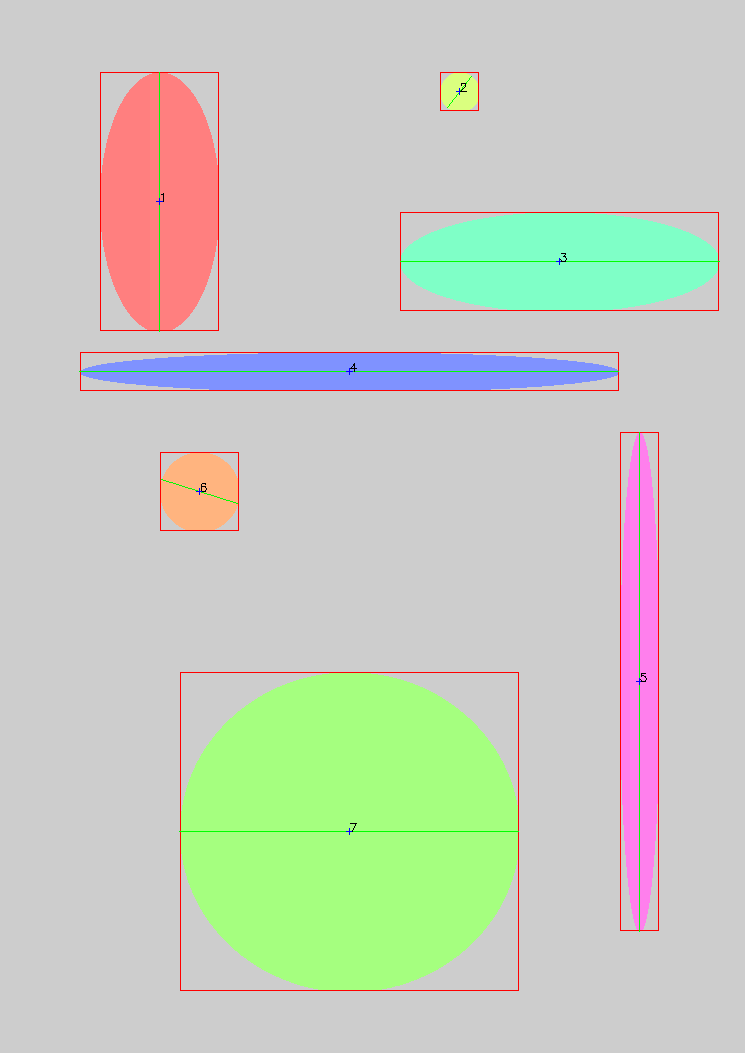
\includegraphics[scale=0.2]{img/blobsDetectados.png}\label{fig:entradafiltrocirc}}
        \hspace{5 mm}
        \subfloat[Salida - Filtro Circular.]{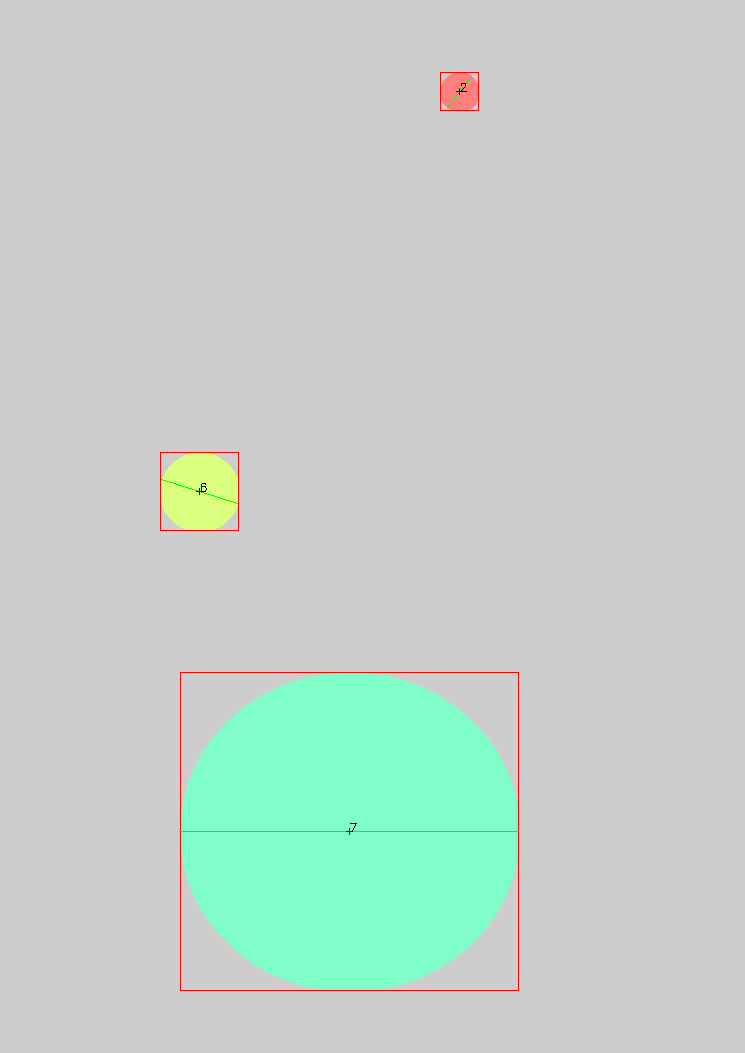
\includegraphics[scale=0.2]{img/circulosDetectados.png}\label{fig:salidafiltrocirc}}
  \caption{Entrada y salida del bloque \emph{filtro circular} para las constantes $A = 0.1$ y $B = 0.3$.}
      \label{ejemplofiltrocirc}
\end{figure}

Es importante destacar que si este filtro se realiza de forma muy selectiva (esto es, darle un valor muy pequeño a las constantes $A$ y $B$ ), no será posible detectar algunos marcadores ya que debido a varios factores -entre los que se encuentran: características de la captura, tamaño de los marcadores en la imagen, iluminación, ruido, etc.- en la mayoría de los cuadros los marcadores no son círculos perfectos. Por esta misma razón se tuvo que descartar la utilización de un detector de círculos, cómo por ejemplo la \textit{transformada de Hough} \cite{hough}, para la implementación de este bloque. 

En la figura \ref{peladoCircular} se ve el resultado de procesar la imagen \ref{peladoBlobs} con el bloque \emph{Circular Filter}.

\begin{figure}[ht!]
        \hspace{-1cm}
        \subfloat[Objetos detectados - Salida del bloque \emph{Detect blobs}.]{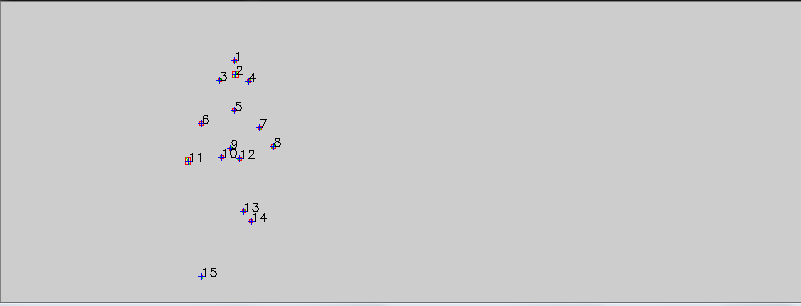
\includegraphics[scale=0.65]{img/peladoFondoAzul_blobs.png}\label{peladoBlobs}}\hspace{3 mm}
        \subfloat[Círculos detectados - Salida del bloque \emph{Circular Filter}.]{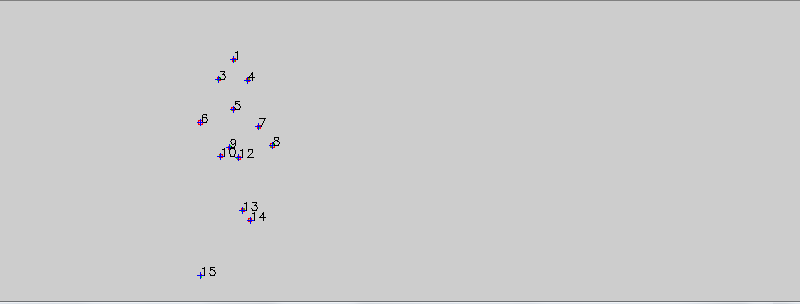
\includegraphics[scale=0.65]{img/peladoFondoAzul_circulos.png}\label{peladoCircular}}
  \caption{Resultado de procesar la imagen \ref{peladoFiltro} con los bloques de detección de blobs y el filtro circular.}
      \label{ejemplocircularfilter}
\end{figure}

Luego del filtro circular, se identifican los blobs que resultaron del filtrado mediante el bloque \emph{Number}, que utiliza la función \emph{cvPutText} de la librería  OpenCV para numerar cada blob de la imagen con su número de \textit{id}. Esta numeración se hace de izquierda a derecha y de arriba hacia abajo.\\


Finalmente, volviendo al diagrama de flujo del bloque general (ver figura \ref{diagramaSegmentacion}), el bloque \emph{Write xml} escribe la posición $(x,y)$ de cada blob en el cuadro procesado, en un archivo XML \cite{xml}. Este bloque es implementado mediante funciones de C++ para escribir archivos, teniendo en cuenta la estructura de los archivos XML.

En la figura \ref{salidaxml}, se presenta un ejemplo del archivo de salida del bloque \emph{Write xml} que corresponde también a la salida del bloque de segmentación. Cómo se observa, es el resultado de analizar una secuencia de tres cuadros (frames 0,1 y 2) donde se detectan 3 marcadores en cada uno de ellos.

\begin{figure}[ht!]
\begin{center}
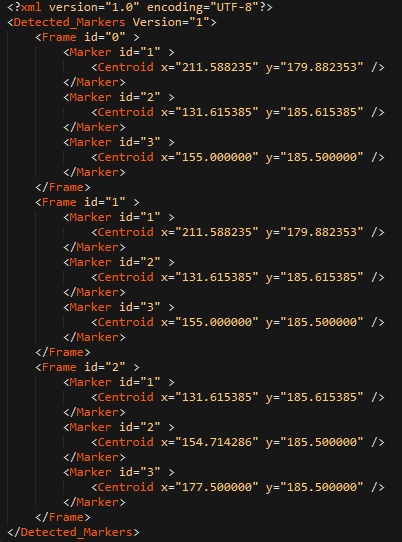
\includegraphics[scale=0.9]{img/salidaXml.png}
\end{center}
\caption{Salida del bloque \emph{Segmentación}.}
\label{salidaxml}
\end{figure}


 Se eligió el formato XML para exportar los resultados porque es un formato conocido universalmente y fácil de importar en cualquier lenguaje, en particular \emph{Matlab} contiene librerías para trabajar con el mismo.

 Resta comentar que, además de los videos a procesar, el algoritmo tiene como entradas opcionales un conjunto de argumentos que establecen distintos parámetros para el procesamiento. Estos argumentos se presentan a continuación:

 \begin{itemize}
\item \textbf{T <valor>} establece un umbral fijo para la umbralización. Debe ser un valor entre 0 y 255.
\item \textbf{A <valor>} área máxima para el filtro por área. Debe ser un valor positivo.
\item \textbf{a <valor>} área mínima para el filtro por área. Debe ser un valor positivo.
\item \textbf{s} guarda los videos que resultan de la salida de los bloques de umbralización y detección de blobs.
 \end{itemize}

\section{Resultados y análisis}
\label{resultadosyanalisissegmentacion}
%hablar de las diferencias entre segmentación sintética y la real, que pasa con la real respecto al ruido, iluminación, etc.
Los resultados para cada marcador se pueden clasificar en 4 tipos:
\begin{itemize}
\item \textit{Verdadero positivo}. Se detecta un marcador dónde hay un marcador realmente.
\item \textit{Verdadero negativo}. No se detecta un marcador dónde no hay un marcador en el cuadro original.
\item \textit{Falso positivo}. Se detecta un marcador dónde en realidad no hay uno.
\item \textit{Falso negativo}. No se detecta marcador dónde hay uno realmente.
\end{itemize}


A raíz de esto, se puede concluir que es deseable tener tanto verdaderos positivos como verdaderos negativos. El falso negativo y el falso positivo corresponden a errores. 

En el desarrollo de sistemas de este tipo, normalmente se priorizan algunos errores frente a otros y se optimiza el sistema para reducir la probabilidad de que ocurran los más prioritarios. Uno de los errores más importantes en segmentación es el \textit{falso negativo}, lo que se traduce en una pérdida de un marcador, ya que si se pierde por muchos cuadros consecutivos es imposible recuperar su trayectoria. 

Otro de los errores a priorizar es el cálculo del centroide de un marcador de forma incorrecta. Esto en general sucede porque al segmentar es complicado detectar el total de los píxeles en un marcador, casi siempre por problemas de iluminación calidad de la filmación, etc.

A continuación, se presentan los resultados de distintas pruebas realizadas en los bloques más críticos que integran la segmentación y detección de marcadores.

\subsection{Umbralización}

Para el bloque de umbralización de este sistema se observó que el resultado obtenido, como era de esperarse, depende fuertemente de las condiciones de captura y obviamente del umbral calculado. 

Para el caso sintético, cómo el que se muestra en la figura \ref{resUmbralizacion}, dónde se imponen las condiciones de captura como es deseable, los resultados fueron muy buenos. Esto es razonable ya que como se vio anteriormente, el método de Otsu calcula el umbral óptimo, por lo que mientras en la imagen se presenten los marcadores cómo los objetos más brillantes y se aprecie un alto contraste entre los mismos y el resto de los elementos (fondo, paciente, etc.), la segmentación será muy efectiva.

\begin{figure}[ht!]
       \hspace{-1cm}
        \subfloat[Captura original de una secuencia sintética.]{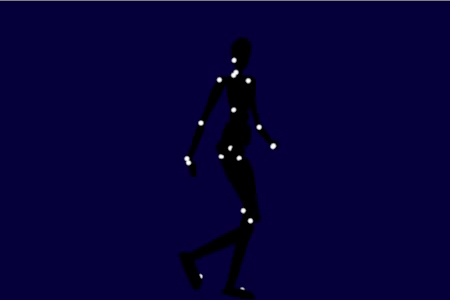
\includegraphics[scale=0.65]{img/peladoFondoAzul.png} %\label{peladoOriginalres}
        }\hspace{1 mm}
        \subfloat[Imagen filtrada con el umbral de Otsu.]{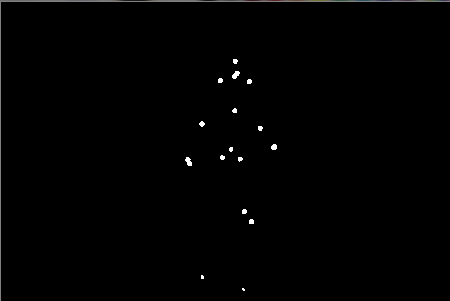
\includegraphics[scale=0.65]{img/peladoFondoAzul_filtro.png}\label{peladoFiltrores}}
  \caption{Entrada y salida del bloque de umbralización para una secuencia sintética.}
      \label{resUmbralizacion}
\end{figure}

Sin embargo, al probar con capturas reales los resultados cambian. En la figura \ref{abelvideo} se muestra un cuadro perteneciente a una captura real, cuyo resultado al pasar por el bloque de umbralización se observa en la figura \ref{abelfiltro}. 

\begin{figure}[ht!]
        \hspace{-1cm}
        \subfloat[Captura original de una secuencia real.]{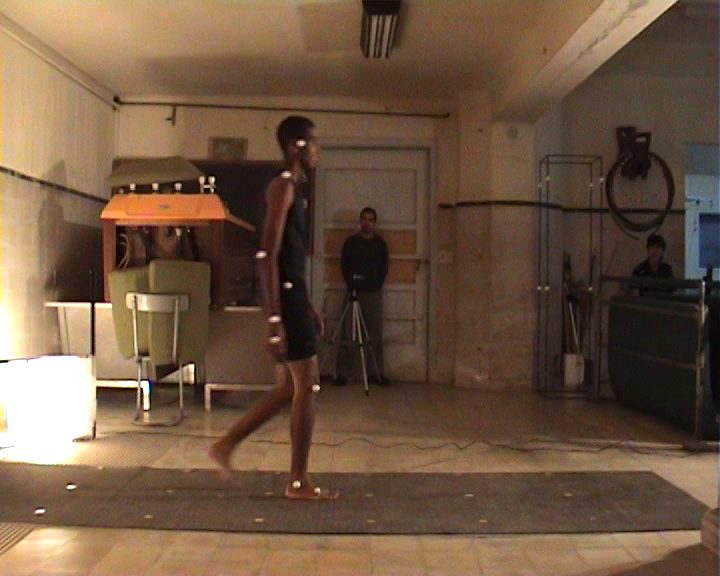
\includegraphics[scale=0.31]{img/abel_original_video.png}\label{abelvideo}}\hspace{1 mm}
        \subfloat[Imagen filtrada con el umbral de Otsu.]{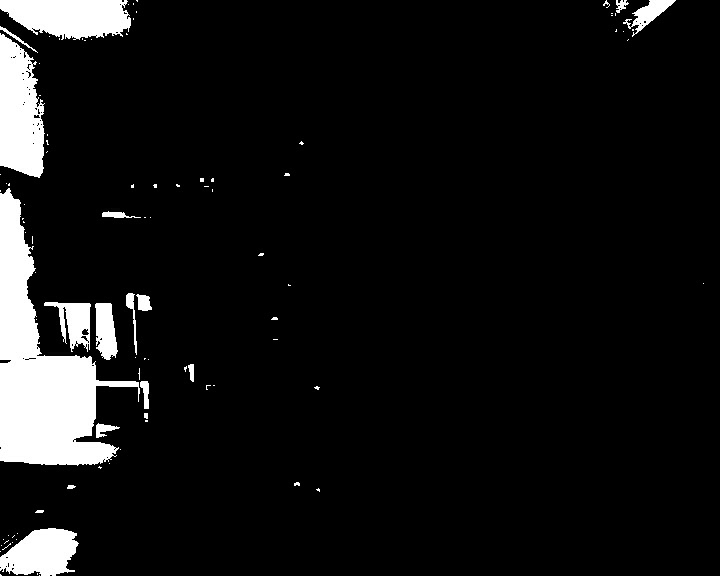
\includegraphics[scale=0.31]{img/abel_original_filtro.png}\label{abelfiltro}}
  \caption{Entrada y salida del bloque umbralización para un caso real.}
      \label{ejemploabelumbr}
\end{figure}

Se puede observar que los objetos resultantes de la segmentación no solamente son los que corresponden a los marcadores, sino que también se presentan otro tipo de objetos de igual o mayor intensidad luminosa. De todos modos, en principio esto no sería un problema, ya que con los filtros que se aplican a continuación de este bloque se podría eliminar el resto de los objetos. Sin embargo ocurre otro problema, que se explicará más adelante.

Otra alternativa para eliminar los objetos detectados que no son marcadores, directamente en esta etapa, es eliminar el fondo mediante un extractor de fondo. En la imagen \ref{abelvideosf} se muestra el cuadro de la figura \ref{abelvideo} luego de extraerle el fondo con un programa de la base de datos \emph{Humaneva} \cite{humanevaBase} implementado en \emph{Matlab}. En la figura \ref{abelfiltrosf} se observan los resultados de aplicarle umbralización a dicha imagen.

\begin{figure}[ht!]
        \hspace{-1cm}
        \subfloat[Captura con el fondo extraído.]{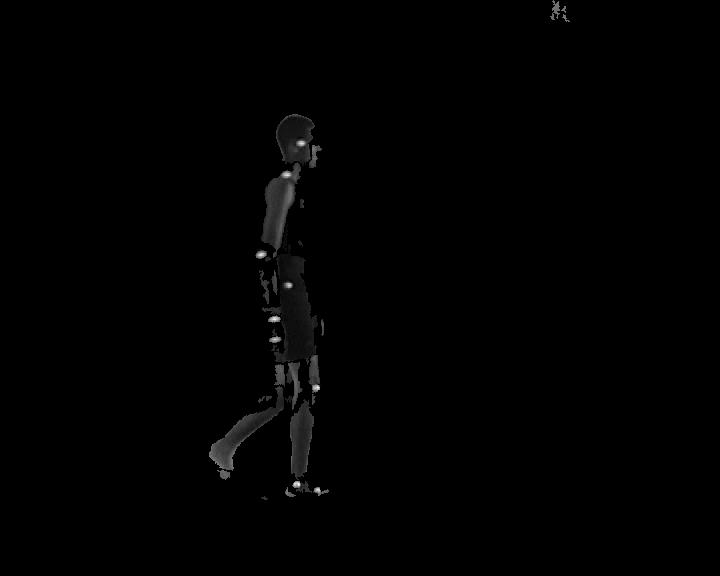
\includegraphics[scale=0.31]{img/abel_sf_video.png}\label{abelvideosf}}\hspace{1 mm}
        \subfloat[Video Filtrado.]{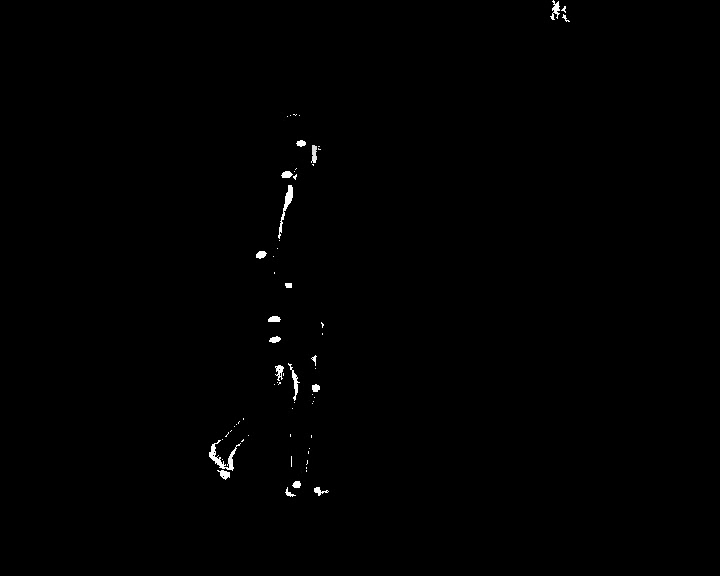
\includegraphics[scale=0.31]{img/abel_sf_filtro.png}\label{abelfiltrosf}}
  \caption{Segmentación para un caso real sin fondo.}
      \label{ejemploabelsf}
\end{figure}

Se observa que, si bien se siguen detectando objetos que no corresponden a los marcadores, el ruido en la imagen filtrada es mucho menor y los marcadores están mejor detectados que en la imagen \ref{abelfiltro}.

\subsection{Detección de marcadores}

Como se mencionó en la explicación del algoritmo, tanto la función para detectar objetos cómo la función para filtrar los mismos por su tamaño son funciones pertenecientes a la librería OpenCV, por lo que no sería necesario probarlas individualmente. En consecuencia, para la detección de marcadores será necesario realizar pruebas más que nada en el filtro circular.

En la figura \ref{ejemplofiltrocirc} se mostraba un ejemplo de funcionamiento de este filtro, dónde se puede ver que a grandes rasgos el filtro funciona correctamente. 

En la figura \ref{ejemplodetectCirculos} se muestra un filtrado más complejo. Se puede observar que para las constantes $A=0.3$ y $B=0.1$ se detectan los círculos correctamente y se incluyen objetos - como el número 19, 29 o 31 - que si bien no son círculos, podrían ser marcadores que por distintos factores (como ser iluminación, calidad de la cámara, ruido, etc.) quedaron segmentados con otra forma. Por otro lado, hay objetos en la imagen \ref{circulosBlobsdetectados2} (por ejemplo el número 28), que también podrían ser un marcador mal detectado, pero no es incluido en la figura \ref{circulosDetectados2}.


\begin{figure}[ht!]
        
        \subfloat[Imagen de prueba.]{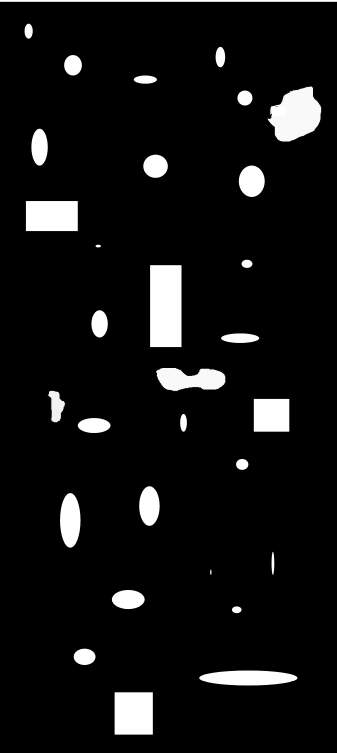
\includegraphics[scale=0.35]{img/circulos2.png}\label{circulos2}}\hspace{2 mm}
        \subfloat[Blobs detectados.]{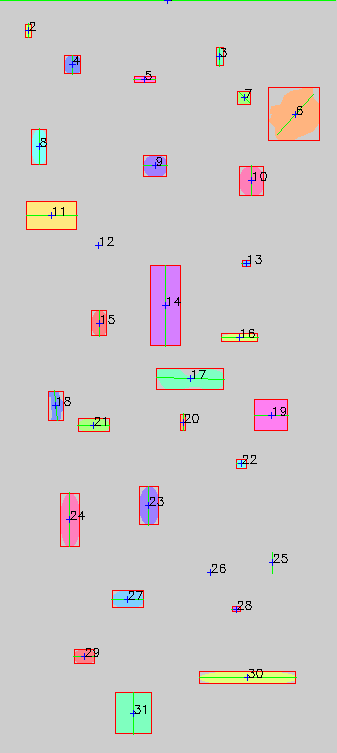
\includegraphics[scale=0.35]{img/blobsDetectados2.png}\label{circulosBlobsdetectados2}}\hspace{2 mm}
        \subfloat[Circulos detectados.]{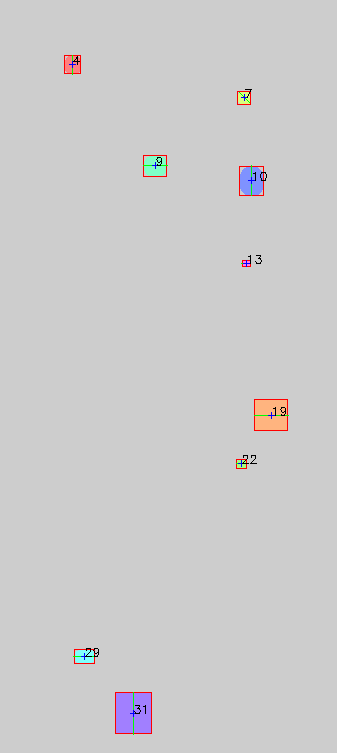
\includegraphics[scale=0.35]{img/circulosDetectados2.png}\label{circulosDetectados2}}
  \caption{Ejemplo de detección de blobs y filtro circular con $A=0.3$, $B=0.1$ para una imagen de prueba.}
      \label{ejemplodetectCirculos}
\end{figure}

Algo parecido a lo comentado en el párrafo anterior sucede con la detección de marcadores en la captura mostrada en la figura \ref{ejemploabelumbr}. Cómo se comentaba anteriormente, en la salida de la umbralización se segmentaron otros objetos además de los marcadores, que se presentan como ruido en la imagen. Para eliminar los objetos más grandes que los marcadores se aplicó el filtro de área estableciendo un área máxima de 50 píxeles (ver figura \ref{abelblobs}). Por otro lado, no es recomendable aplicar un filtro de área mínima ya que los marcadores segmentados resultaron ser muy pequeños, por lo que de establecer esta cota inferior probablemente se eliminarán algunos. Lo mismo pasa con la aplicación de difuminado (o \textit{smoothing}): si bien este proceso es muy efectivo para eliminar ruido en los bordes, resulta ser contraproducente cuando los marcadores son muy pequeños, ya que también los elimina.

Cómo se puede ver en la figura \ref{abelcirculos} los resultados para esta captura no fueron muy buenos ya que, como los marcadores detectados presentan un área de unos pocos píxeles, el filtro circular no fue capaz de reconocerlos como círculos.  

\begin{figure}[ht!]
        \hspace{-1cm}
        \subfloat[Blobs detectados.]{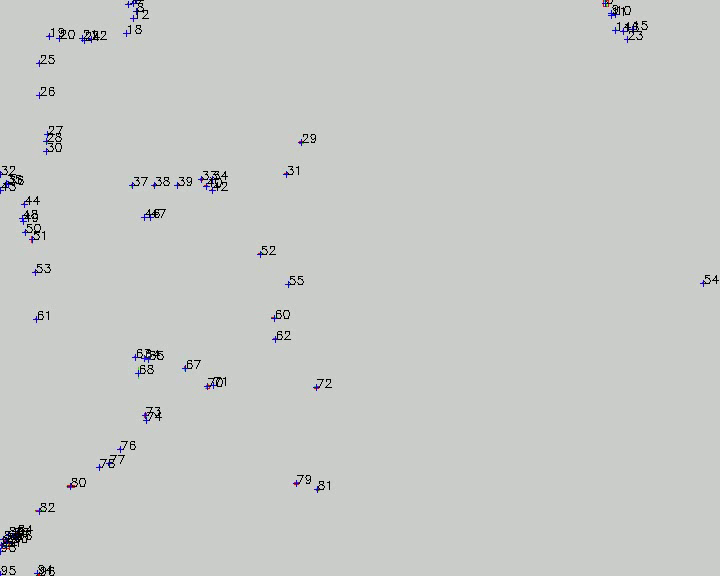
\includegraphics[scale=0.31]{img/abel_original_blobs.png}\label{abelblobs}}\hspace{1 mm}
        \subfloat[Circulos detectados.]{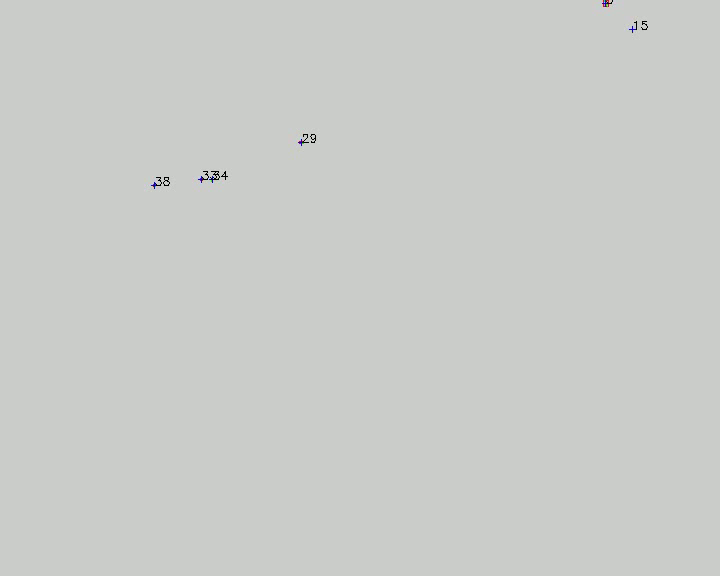
\includegraphics[scale=0.31]{img/abel_original_circulos.png}\label{abelcirculos}}
  \caption{Detección de marcadores para un caso real, con $A=0.3$, $B=0.1$ y área máxima de $50$ píxeles}
      \label{ejemploabeldet}
\end{figure}

Por otro lado, para el caso real pero sin fondo (figura \ref{ejemploabelsf}), se puede ver en la figura \ref{ejemploabel} que no se detecta tanto ruido como en el caso anterior. Sin embargo, los círculos detectados en la figura \ref{abelcirculossf} vuelven a ser muy pocos, dejando marcadores fuera de la detección.

\begin{figure}[ht!]
        \hspace{-1cm}
        \subfloat[Blobs detectados.]{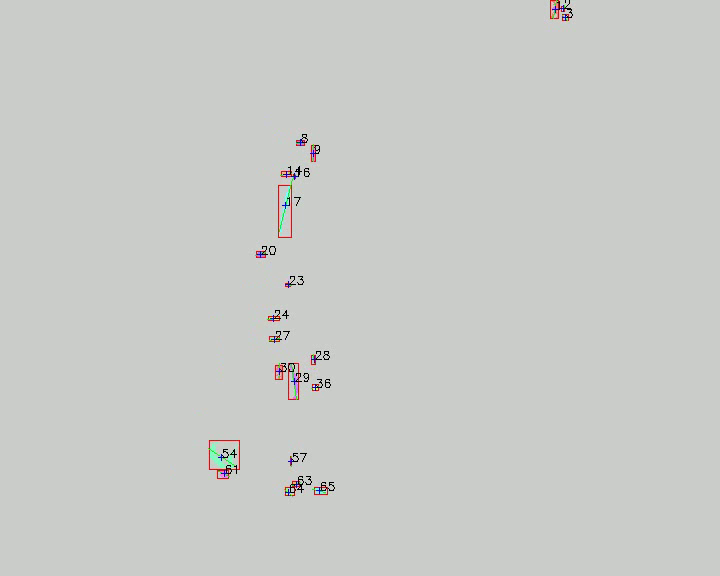
\includegraphics[scale=0.31]{img/abel_sf_blobs.png}\label{abelblobssf}}\hspace{1 mm}
        \subfloat[Círculos detectados.]{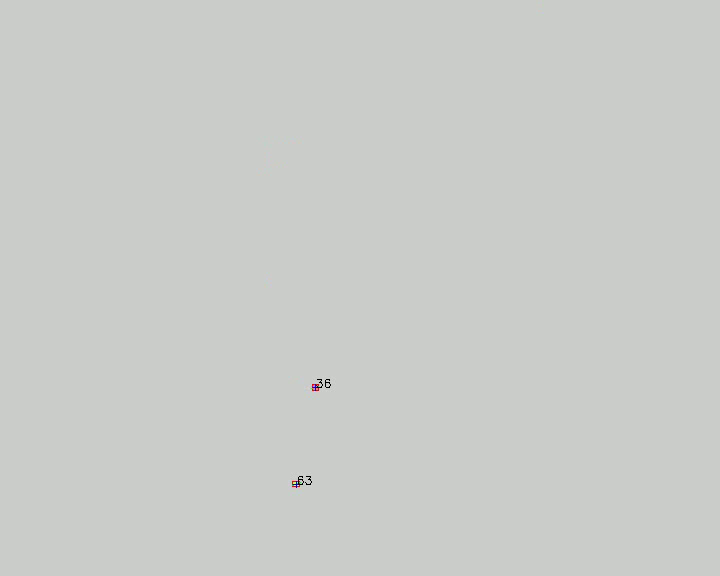
\includegraphics[scale=0.31]{img/absel_sf_circulos.png}\label{abelcirculossf}}
  \caption{Segmentación y detección de marcadores para un caso real sin fondo, con $A=0.3$, $B=0.1$ y área mínima de $10$ píxeles}
      \label{ejemploabel}
\end{figure}

Si se observa la figura \ref{abelfiltrosf} se puede apreciar que los marcadores están segmentados con una superficie mayor a la de la figura \ref{abelfiltro}.  Esto da como indicio que para esta captura (con estas condiciones de iluminación, ambiente, paciente, etc.) el filtro circular con valores en sus constantes de $A=0.3$ y $B=0.1$ está siendo muy selectivo.

Aumentando estos valores a por ejemplo $A=0.5$ y $B=0.4$, se puede observar que la detección mejora, incluyendo más marcadores -\textit{verdaderos positivos}- en la salida (ver figura \ref{ejemploabel2}).

\begin{figure}[ht!]
        \hspace{-1cm}
        \subfloat[Blobs detectados.]{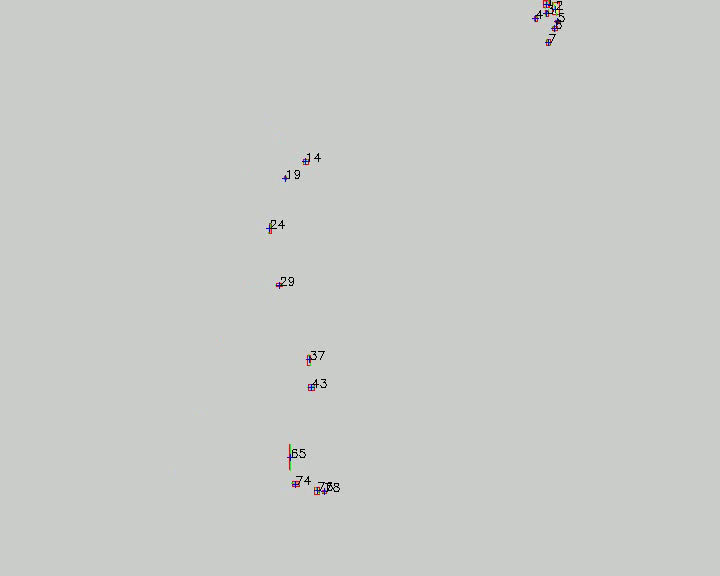
\includegraphics[scale=0.31]{img/abel_sf_blobs_2.png}\label{abelblobssf2}}\hspace{1 mm}
        \subfloat[Circulos detectados.]{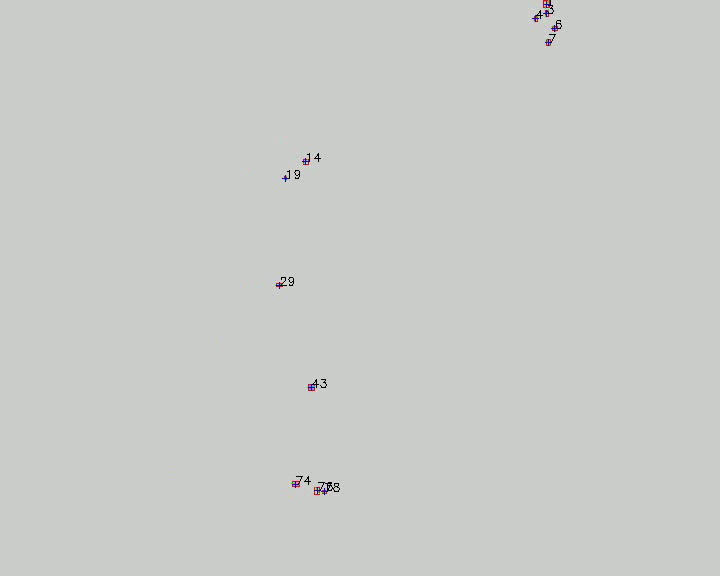
\includegraphics[scale=0.31]{img/abel_sf_circulos_2.png}\label{abelcirculossf2}}
  \caption{Segmentación y detección de marcadores para el caso de la figura \ref{ejemploabelsf} , con $A=0.5$, $B=0.4$, área mínima de $10$ píxeles y área máxima de $50$ píxeles}
      \label{ejemploabel2}
\end{figure}

Para el caso sintético, hacer el análisis anterior no tiene el mismo provecho, ya que al obtenerse una segmentación muy buena los marcadores se detectaron en su totalidad (ver figura \ref{peladoBlobssint}). 

Por otro lado, en la figura \ref{peladoCircularsint} puede verse que el filtro circular detecta todos los marcadores, a excepción de los que están superpuestos entre si (como el 2 y el 11 de la figura \ref{peladoBlobssint}), ya que al superponerse pierden la forma circular.

 Queda cómo tarea pendiente para una etapa futura optimizar el bloque de segmentación para estos casos particulares, de forma tal de no perder los datos de los marcadores superpuestos. Una posible solución podría ser utilizar el método de erosión, para separar los marcadores y quedarse con la posición de sus centroides.

\begin{figure}[H]
        \hspace{-1cm}
        \subfloat[Blobs detectados.]{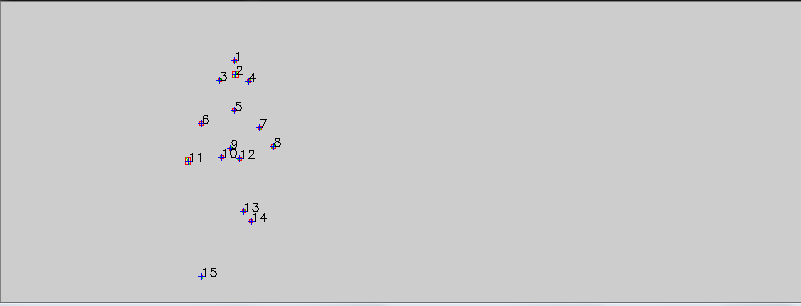
\includegraphics[scale=0.67]{img/peladoFondoAzul_blobs.png}\label{peladoBlobssint}}\hspace{1 mm}
        \subfloat[Círculos detectados.]{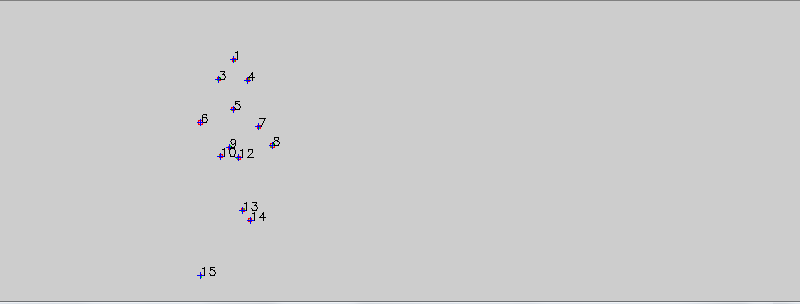
\includegraphics[scale=0.67]{img/peladoFondoAzul_circulos.png}\label{peladoCircularsint}}
  \caption{Resultado de procesar la imagen \ref{peladoFiltrores} con los bloques de detección de blobs y el filtro circular.}
      \label{detectMarcadoresSinteticos}
\end{figure}

\subsection{Medida de error}

Como se mencionó anteriormente, una de las ventajas de tener una base de datos sintética, es poder tener un \textit{ground truth} contra el cual comparar los resultados obtenidos con el sistema implementado. En la figura \ref{ejMedErr}, se observa la comparación de la segmentación de una secuencia contra su ground truth para un sujeto moviéndose de izquierda a derecha.
\vspace{-3mm}
\begin{figure}[ht!]
\begin{center}
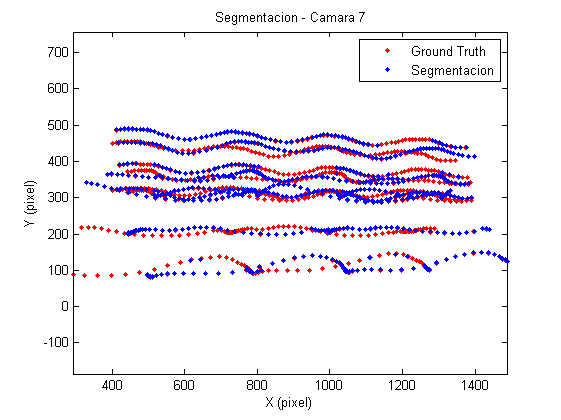
\includegraphics[scale=0.6]{img/imagen_segmentacion_cam7_8_07_100_200.png}
\end{center}
\vspace{-7mm}
\caption{Segmentación de cámara 7 y ground truth.}
\label{ejMedErr}
\end{figure}

En el cuadro \ref{tablaerrorseg} se puede observar una medida de error para una secuencia sintética estándar de la base. En ella se observa, para cada cámara, el porcentaje de detección de marcadores en toda la captura, el error promedio en píxeles y el percentil 99\footnote{Valor del error en píxeles por debajo del cual se encuentra el 99\% de los marcadores.} también en píxeles Se realizaron estas medidas para varias secuencias distintas y los valores se mantienen aproximadamente en este mismo rango.

\begin{table}[H]
\centering
\begin{tabular}{@{}cccc@{}}
\toprule
\multicolumn{1}{l}{Id de cámara} & \begin{tabular}[c]{@{}c@{}}Porcentaje\\  de detección\end{tabular} & \begin{tabular}[c]{@{}c@{}}Error promedio\\ (píxeles)\end{tabular} & \begin{tabular}[c]{@{}c@{}}Percentil 99\\ (píxeles)\end{tabular} \\ \midrule
1                           & 73.31\%                                                            & 0.9121                                                             & 2.2751                                                           \\
2                           & 86.22\%                                                            & 0.9477                                                             & 3.6592                                                           \\
3                           & 67.36\%                                                            & 1.0278                                                             & 3.4376                                                           \\
4                           & 65.79\%                                                            & 1.0343                                                             & 3.5561                                                           \\
5                           & 63.97\%                                                            & 0.9965                                                             & 2.529                                                            \\
6                           & 63.85\%                                                            & 0.9822                                                             & 2.4508                                                           \\
7                           & 59.59\%                                                            & 1.0388                                                             & 3.4561                                                           \\
8                           & 57.21\%                                                            & 1.0713                                                             & 3.7559                                                           \\
9                           & 59.09\%                                                            & 1.0206                                                             & 2.927                                                            \\
10                          & 77.44\%                                                            & 1.0441                                                             & 3.3186                                                           \\
11                          & 57.83\%                                                            & 1.0316                                                             & 3.8255                                                           \\
12                          & 56.83\%                                                            & 1.0561                                                             & 4.3085                                                           \\
13                          & 60.28\%                                                            & 1.0121                                                             & 2.6783                                                           \\
14                          & 63.97\%                                                            & 0.9931                                                             & 2.536                                                            \\
15                          & 64.91\%                                                            & 0.9948                                                             & 2.5073                                                           \\
16                          & 64.6\%                                                             & 0.9994                                                             & 3.126                                                            \\
17                          & 64.97\%                                                            & 1.0094                                                             & 2.9885                                                           \\ \bottomrule
\end{tabular}
\caption{Medida de error en captura estándar de la base de datos sintética.}
\label{tablaerrorseg}
\end{table}

En la figura \ref{histerr} se observa un histograma que contempla datos de todas las cámaras a lo largo de la secuencia completa, dónde se muestra la cantidad de marcadores por rango de error en píxeles. Observando la figura se puede ver que la curva tiene una media en el rango de 1 píxel de error.  

\begin{figure}[H]
\begin{center}
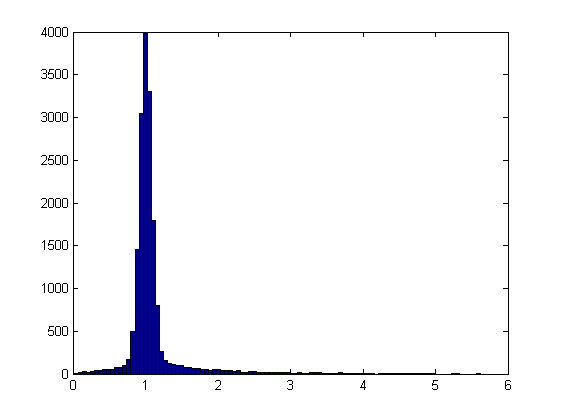
\includegraphics[scale=0.6]{img/Histo_Error.png}
\end{center}
\vspace{-1cm}
\caption{Histograma de cantidad de marcadores por rango de error en píxeles}
\label{histerr}
\end{figure}

Este cálculo es realizado para una secuencia de 110 cuadros, con 17 cámaras y 13 marcadores en el cuerpo del paciente. Sin embargo, el total de marcadores en el histograma no son $17*13*113 = 24973$ debido a que en cada cámara no se visualizan todos los marcadores. Para ver el total de los marcadores analizados hay que tener en cuenta el porcentaje de detección de cada cámara, esto da un total de $15671$ marcadores.

 Más adelante, se explicará en detalle el método utilizado para calcular el error de la tabla \ref{tablaerrorseg}.

Finalmente, a modo de conclusión, se puede decir que el bloque de segmentación y detección de marcadores funciona correctamente para secuencias sintéticas como las de la base de datos, teniendo errores promedio de 1 píxel y errores máximos de 4 píxeles. Estos errores se mantienen en el rango de los errores de los otros bloques que componen el sistema, por lo que podría decirse que, si bien se utilizaron métodos de segmentación sencillos y no tan robustos como otros métodos, los resultados se mantienen acordes a la performance general de esta primer versión del sistema.

Por otro lado, en las pruebas con secuencias reales no se dieron resultados tan buenos, sin embargo ajustando los parámetros de forma adecuada se puede ver que se logran detectar un número razonable de marcadores por cámara. Además, no hay que pasar por alto que no fue fácil conseguir capturas reales para probar este bloque, y las que se obtuvieron no se adaptan del todo a las hipótesis del problema.

 Queda pendiente como posible mejora a futuro robustecer este bloque, de forma tal de poder detectar marcadores en otros contextos no tan amigables como las condiciones del laboratorio establecidas para esta primera etapa de desarrollo.